%%%%%%%%%%%%%%%%%%%%%%%%%%%%%%%%%%%%%%%%%
% Short Sectioned Assignment
% LaTeX Template
% Version 1.0 (5/5/12)
%
% This template has been downloaded from:
% http://www.LaTeXTemplates.com
%
% Original author:
% Frits Wenneker (http://www.howtotex.com)
%
% License:
% CC BY-NC-SA 3.0 (http://creativecommons.org/licenses/by-nc-sa/3.0/)
%
%%%%%%%%%%%%%%%%%%%%%%%%%%%%%%%%%%%%%%%%%

%----------------------------------------------------------------------------------------
%	PACKAGES AND OTHER DOCUMENT CONFIGURATIONS
%----------------------------------------------------------------------------------------

\documentclass[paper=a4, fontsize=11pt]{scrartcl} % A4 paper and 11pt font size 

\usepackage[T1]{fontenc} % Use 8-bit encoding that has 256 glyphs
\usepackage[english]{babel} % English language/hyphenation
\usepackage{amsmath,amsfonts,amsthm} % Math packages

\usepackage{sectsty} % Allows customizing section commands
%\allsectionsfont{\centering \normalfont\scshape} % Make all sections centered, the default font and small caps

\usepackage{fancyhdr} % Custom headers and footers
\pagestyle{fancyplain} % Makes all pages in the document conform to the custom headers and footers
\fancyhead{} % No page header - if you want one, create it in the same way as the footers below
\fancyfoot[L]{} % Empty left footer
\fancyfoot[C]{} % Empty center footer
\fancyfoot[R]{\thepage} % Page numbering for right footer
\renewcommand{\headrulewidth}{0pt} % Remove header underlines
\renewcommand{\footrulewidth}{0pt} % Remove footer underlines
\setlength{\headheight}{13.6pt} % Customize the height of the header

\numberwithin{equation}{section} % Number equations within sections (i.e. 1.1, 1.2, 2.1, 2.2 instead of 1, 2, 3, 4)
\numberwithin{figure}{section} % Number figures within sections (i.e. 1.1, 1.2, 2.1, 2.2 instead of 1, 2, 3, 4)
\numberwithin{table}{section} % Number tables within sections (i.e. 1.1, 1.2, 2.1, 2.2 instead of 1, 2, 3, 4)

\setlength\parindent{0pt} % Removes all indentation from paragraphs - comment this line for an assignment with lots of text

\usepackage{bbm}
\usepackage{graphicx}
\usepackage{xcolor} % For color
\usepackage{subcaption}
\usepackage{booktabs}
%----------------------------------------------------------------------------------------
%	TITLE SECTION
%----------------------------------------------------------------------------------------

\newcommand{\horrule}[1]{\rule{\linewidth}{#1}} % Create horizontal rule command with 1 argument of height

\title{	
\normalfont \normalsize 
\horrule{0.5pt} \\[0.4cm] % Thin top horizontal rule
\huge Assignment Two \\ % The assignment title
\horrule{2pt} \\[0.5cm] % Thick bottom horizontal rule
}

\author{
	Matthew C.~Scicluna\\
	D\'epartement d'Informatique et de Recherche Op\'erationnelle\\
	Universit\'e de Montr\'eal\\
	Montr\'eal, QC H3T 1J4 \\
	\texttt{matthew.scicluna@umontreal.ca}
}


\date{\normalsize\today} % Today's date or a custom date

\begin{document}

\maketitle % Print the title

%----------------------------------------------------------------------------------------
%	PROBLEM 1
%----------------------------------------------------------------------------------------
\section{Fisher LDA}
Given the class variable, the data are assumed to be Gaussians with different means for different classes but with the same covariance matrix.

\subsection{Derive the form of the maximum likelihood estimator for this model}
	Given \(Y \sim Bernoulli(\pi), X \mid Y = j \sim \mathcal{N}(\mu_j, \Sigma) \). We first obtain the log likelihood \(l(\theta \mid D)\), where \(D\) are the data points \(\{x^{(i)}, y^{(i)}\}_{i=1}^N\) and \(\theta = (\pi, \mu_0,\mu_1, \Sigma)\),\ \(\pi \in [0,1]\),\ \(\mu_0,\mu_1 \in \mathbb{R}^d \) and \(\Sigma \in \mathbb{R}^{d \times d} \). We suppose WLOG that \(y^{(1)} = \cdots = y^{(N_0)} = 0 \) for \(N_0<N\) and \(y^{(N_0+1)} = \cdots = y^{(N)} = 1 \). 
	\begin{align*}
	l(\theta \mid D) &= \ln P(D \mid \theta) \\
	&= \sum_{i=1}^{N} \ln P(x^{(i)}, y^{(i)} \mid \theta) \\ 
	&= \sum_{i=1}^{N} \ln P(x^{(i)} \mid y^{(i)} \mid \theta) + \ln P(y^{(i)} \mid \theta)\\
	& \propto -\frac{N}{2}\ln |\Sigma| -\frac{1}{2} \sum_{i=1}^{N_0}  (x^{(i)}-\mu_{0})^T\Sigma^{-1}(x^{(i)}-\mu_{0}) -\frac{1}{2} \sum_{i=N_0 + 1}^{N}  (x^{(i)}-\mu_{1})^T\Sigma^{-1}(x^{(i)}-\mu_{1}) \\
	&+ (N-N_0)\ln \pi + N_0\ln(1-\pi)
	\end{align*}
	
\subsubsection{MLE of \(\pi\)}
	
	To get the MLE of \(\pi\), we find the stationary points of \(l(\theta \mid D)\):
	\begin{align*}
	\frac{\partial l(\theta \mid D)}{\partial \pi} &= \frac{\partial}{\partial \pi} (N-N_0)\ln \pi + N_0\ln(1-\pi) \\
	&=  \frac{N-N_0}{\pi} - \frac{N_0}{1 - \pi}
	\end{align*}
	Setting this to \(0\) yields:
	\begin{align*}
	\frac{N-N_0}{\pi} = \frac{N_0}{1 - \pi} \Rightarrow N\pi = N - N_0 \Rightarrow \pi = \frac{N-N_0}{N}
	\end{align*}
	We can confirm that this is a minimum since
	\begin{align*}
	\frac{\partial^2 l(\theta \mid D)}{\partial \pi^2} = -\frac{N-N_0}{\pi^2}-\frac{N_0}{(1-\pi)^2} < 0
	\end{align*}

\subsubsection{MLE of \(\mu_0, \mu_1\)}

	We look for stationary points for candidate MLE solutions of \(\mu_0\).
	\begin{align}
	\frac{\partial l(\theta \mid D)}{\partial \mu_0} &= \sum_{j=1}^{N_0} -\frac{1}{2} \frac{\partial}{\partial \mu_0} (x^{(j)}-\mu_0)^T\Sigma^{-1}(x^{(j)}-\mu_0)
	\end{align}
	To solve this, we use the chain rule. Let \(f: \mathbb{R}^d \rightarrow \mathbb{R}^d\), \(f(x) = x-\mu_0\) and let \(g: \mathbb{R}^d \rightarrow \mathbb{R}\), \(g(x) = x^T\Sigma^{-1}x\) where \(\Sigma^{-1}\) is symmetric and positive semi definite.
	From lecture results we have that \(d_f(x) = I\) and \(d_g(x) = 2x^T\Sigma^{-1}\). We can then compute 
	\begin{align}
	d_{g \circ f}(x) &= d_{g} (f(x)) \cdot d_{f} (x) = 2(x-\mu_0)^T\Sigma^{-1}\cdot I
	\end{align}
	
	Upon substituting (1.2) into (1.1) and equating to zero we have that:
	\begin{align}
	\frac{\partial l(\theta \mid D)}{\partial \mu_0} &= \sum_{j=1}^{N_0} -((x^{(j)}-\mu_0)^T\Sigma^{-1})^T = \Sigma^{-1}(x^{(j)}-\mu_0)= 0
	\end{align}
	We left multiply each side by \((\Sigma^{-1})^{-1}\) (which exists since \(\Sigma^{-1}\) symmetric and positive definite), and get:
	\begin{align}
	\sum_{j=1}^{N_0} -(x^{(j)}-\mu_0) = 0 \Rightarrow \mu_0 = \frac{1}{N_0}\sum_{j=1}^{N_0} x^{(j)} = \bar{x}_0
	\end{align}
	An identical computation yields \(\mu_1 = \frac{1}{N - N_0}\sum_{j=N_0+1}^{N} x^{(j)} = \bar{x}_1\). Hence the MLE estimates for each class mean is the sample mean of each class.
	
\subsubsection{MLE of \(\Sigma\)}
	We compute the MLE for \(\Sigma^{-1}\) instead of for \(\Sigma\) using the invariance of the MLE. We substitue the MLE estimate for \(\mu_0, \mu_1\).
	
	\begin{align*}
	\frac{\partial l(\theta \mid D)}{\partial \Sigma^{-1}} =
		\frac{\partial}{\partial \Sigma^{-1}}\left(\frac{-N}{2}\ln |\Sigma| -\frac{1}{2} \sum_{i=1}^{N_0} (x^{(i)}-\bar{x}_0)^T\Sigma^{-1}(x^{(i)}-\bar{x}_0) -\frac{1}{2} \sum_{i=N_0 + 1}^{N}  (x^{(i)}-\bar{x}_1)^T\Sigma^{-1}(x^{(i)}-\bar{x}_1) \right)
	\end{align*}
	
	Differentiating the first term yields
	\begin{align}
	\frac{\partial}{\partial \Sigma^{-1}}\ln |\Sigma|
	&=\frac{\partial}{\partial \Sigma^{-1}}-\ln |\Sigma^{-1}|\\
	&=-\Sigma
	\end{align}
	Where the derivative evaluated in (1.6) comes from a result proved in class.
	
	Differentiating the second term yields: 
	\begin{align}
	\frac{\partial}{\partial \Sigma^{-1}}\sum_{i=1}^{N_0}  (x^{(i)}-\bar{x}_0)^T\Sigma^{-1}(x^{(i)}-\bar{x}_0)
	&= \frac{\partial}{\partial \Sigma^{-1}}\sum_{i=1}^{N_0}  tr\left((x^{(i)}-\bar{x}_0)^T\Sigma^{-1}(x^{(i)}-\bar{x}_0)\right) \\
	&= \frac{\partial}{\partial \Sigma^{-1}}\sum_{i=1}^{N_0} tr\left( (x^{(i)}-\mu_{0}) (x^{(i)}-\mu_{0})^T\Sigma^{-1}\right) \\
	&= \frac{\partial}{\partial \Sigma^{-1}} tr\left( \sum_{i=1}^{N_0} (x^{(i)}-\mu_{0}) (x^{(i)}-\mu_{0})^T\Sigma^{-1}\right)
	\end{align}
	
	Where (1.7) is using that a scalar is the Trace of a 1D matrix, (1.8) uses that the Trace is invariant under cyclic permutations, and (1.9) uses that the Trace is a linear operator.
	
	Finally, if we let \(S_0 = \frac{1}{N_0}\sum_{i=1}^{N_0} (x^{(i)}-\mu_{0}) (x^{(i)}-\mu_{0})^T\) we can rewrite (1.9) as
	\begin{align}
	\frac{\partial}{\partial \Sigma^{-1}}\sum_{i=1}^{N_0}  (x^{(i)}-\bar{x}_0)^T\Sigma^{-1}(x^{(i)}-\bar{x}_0) &= \frac{\partial}{\partial \Sigma^{-1}} N_0tr\left(S_0\Sigma^{-1}\right) \\
	&= N_0S_0
	\end{align}
	An equivalent computation yields:
	\begin{align}
	& \frac{\partial}{\partial \Sigma^{-1}}\sum_{i=N_0 + 1}^{N}  (x^{(i)}-\bar{x}_1)^T\Sigma^{-1}(x^{(i)}-\bar{x}_1) \\
	&= \frac{\partial}{\partial \Sigma^{-1}} (N-N_0)tr\left(S_1\Sigma^{-1}\right) \\
	&= (N-N_0)S_1
	\end{align}
	Where \(S_1 = \frac{1}{N-N_0}\sum_{i=N_0+1}^{N} (x^{(i)}-\mu_{1}) (x^{(i)}-\mu_{1})^T\).
	Susbtituting the results from (1.6), (1.10) and (1.11) into the derivative with respect to \(\Sigma^{-1}\) we have that:
	\begin{align}
	\frac{\partial l(\theta \mid D)}{\partial \Sigma^{-1}} &= \frac{N}{2}\Sigma -\frac{1}{2}N_0S_0  -\frac{1}{2}(N-N_0)S_1
	\end{align}
	
	And so \( \frac{\partial l(\theta \mid D)}{\partial \Sigma^{-1}} = 0 \Rightarrow N\Sigma =N_0S_0  +(N-N_0)S_1 \Rightarrow \Sigma = \frac{N_0}{N}S_0 + \frac{N-N_0}{N}S_1 \).
	
	We leave the proof that the stationary points are maxima to the reader.
	
	\subsection{Derive \(p(y = 1|x)\)}
	
	\begin{align}
	p(y = 1|x) &= \frac{p(x | y = 1)p(y=1)}{p(x | y = 0)p(y=0) + p(x | y = 1)p(y=1)}\\
	&= \frac{\pi e^{\left\{-\frac{1}{2}(x-\mu_1)^T\Sigma^{-1}(x-\mu_1)\right\}}}{
	(1 - \pi) e^{\left\{-\frac{1}{2}(x-\mu_0)^T\Sigma^{-1}(x-\mu_0)\right\}} + \pi e^{\left\{-\frac{1}{2}(x-\mu_1)^T\Sigma^{-1}(x-\mu_1)\right\}}}\\
	&= \frac{\pi e^{\left\{-\frac{1}{2}(x-\mu_1)^T\Sigma^{-1}(x-\mu_1)\right\}}}{
	(1 - \pi) e^{\left\{-\frac{1}{2}(x-\mu_0)^T\Sigma^{-1}(x-\mu_0)\right\}} + \pi e^{\left\{-\frac{1}{2}(x-\mu_1)^T\Sigma^{-1}(x-\mu_1)\right\}}} \\
	&= \frac{e^{\left\{\ln\pi-\mu_1^T\Sigma^{-1}x -\frac{1}{2}\mu_1^T\Sigma^{-1}\mu_1)\right\}}}{
		e^{\left\{\ln(1-\pi)-\mu_0^T\Sigma^{-1}x -\frac{1}{2}\mu_0^T\Sigma^{-1}\mu_0)\right\}}+e^{\left\{\ln\pi-\mu_1^T\Sigma^{-1}x -\frac{1}{2}\mu_1^T\Sigma^{-1}\mu_1)\right\}}
		}
	\end{align}
	Where (1.19) comes from cancelling the quadratic in \(x\) from the numerator and denominator.
	
	If we let
	\begin{equation}
	\beta_0=\begin{bmatrix}
	 -\frac{1}{2}\mu_0^T\Sigma^{-1}\mu_0 + ln(1-\pi)\\
	-\Sigma^{-1}\mu_0 \\
	\end{bmatrix}
	\end{equation}
	and
	\begin{equation}
	\beta_1=\begin{bmatrix}
	-\frac{1}{2}\mu_1^T\Sigma^{-1}\mu_1 + ln(\pi)\\
	-\Sigma^{-1}\mu_1 \\
	\end{bmatrix}
	\end{equation}
	Then if we augment \(x\) to have a first component equal to one, we can rewrite (1.19) as
	\begin{align}
	\frac{e^{\beta_1^Tx}}{e^{\beta_0^Tx}+e^{\beta_1^Tx}}
	\end{align}
	Which we recognize has the same form as a Logistic Regression.
	Upon dividing by \(e^{\beta_1^Tx}\), we get that \(P(y=1 \mid x) = \sigma\left(\beta_0^Tx-\beta_1^Tx\right)\).
	We notice that the decision boundary is linear in \(x\). to find it, we note that \(\sigma(z) = 0.5\) iff \(z = 0\), and so we solve for \(\beta_0^Tx-\beta_1^Tx = 0\). For \((x^1,x^2) \in \mathbb{R}^2\), this would be:
	\begin{align}
	x^2 = -\frac{\beta_0^0-\beta_1^{0} + (\beta_0^{1}-\beta_1^{1})x^1}{\beta_0^{1}-\beta_1^{1}}
	\end{align}
	
	Where \(\beta_i^T := (\beta_i^0, \beta_i^1)\). We evaluating the above using the MLE estimates for 3 datasets to get figure 1.1.
	
	\begin{figure}
	\begin{subfigure}{.5\textwidth}
		\centering
		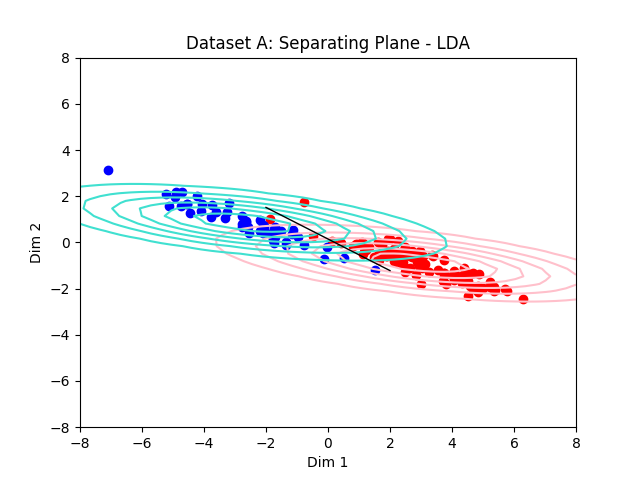
\includegraphics[width=.9\linewidth]{img_A_MoG.png}
	\end{subfigure}
	\begin{subfigure}{.5\textwidth}
		\centering
		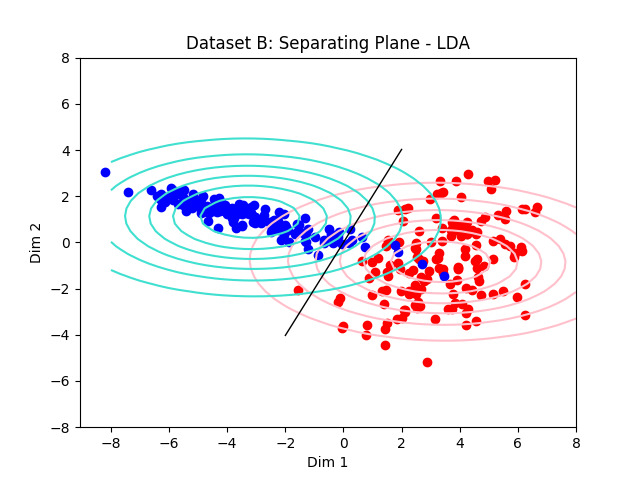
\includegraphics[width=.9\linewidth]{img_B_MoG.png}
	\end{subfigure}
	\begin{subfigure}{.5\textwidth}
		\centering
		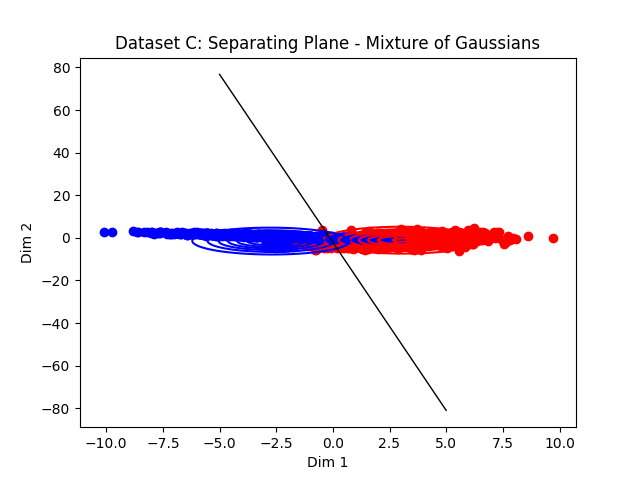
\includegraphics[width=.9\linewidth]{img_C_MoG.png}
	\end{subfigure}
	\caption{Three different Datasets fit with MLE estimates from Mixture of Gaussian models. The seperating plane is in black, and contours from each gaussian are in red and blue.}
	\end{figure}


\section{Logistic Regression}
	We now implement logistic regression to learn an affine function \(f(x) = w^Tx+b\) using the IRLS algorithm applied on each of the above datasets. The learning stopped when the norm of the difference of the parameters fell below 0.001. The estimated parameters are displayed in table 2.1. The corresponding decision boundary is presented in figure 2.1.
	
	\begin{table}
		\caption {Logistic Regression Parameter Values} \label{tab:title} 
		\begin{center}		
			\begin{tabular}{*5l}   
			\toprule
				\emph{Dataset}&  $b$ & $w_1$  & $w_2$\\\midrule
				A & -2.05 & -11.5 & -19.2 \\ 
				B & 1.29 & -1.62 & 0.96 \\
				C & 0.95 & -2.08 & 0.65 \\\bottomrule
				\hline
			\end{tabular}
		\end{center}
	\end{table}
	
	\begin{figure}
		\begin{subfigure}{.5\textwidth}
			\centering
			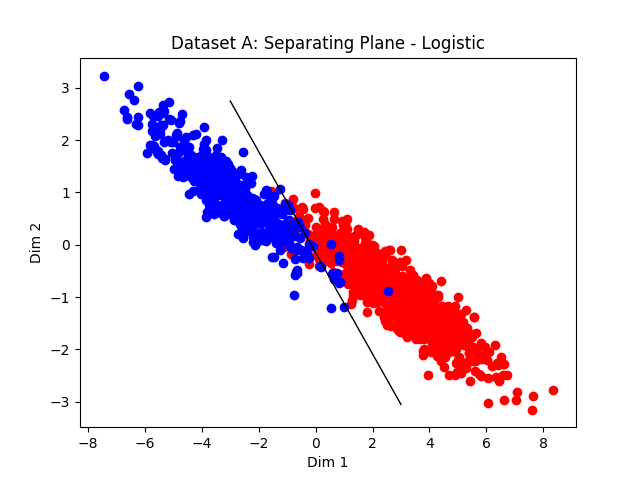
\includegraphics[width=.9\linewidth]{img_A_Log.png}
		\end{subfigure}
		\begin{subfigure}{.5\textwidth}
			\centering
			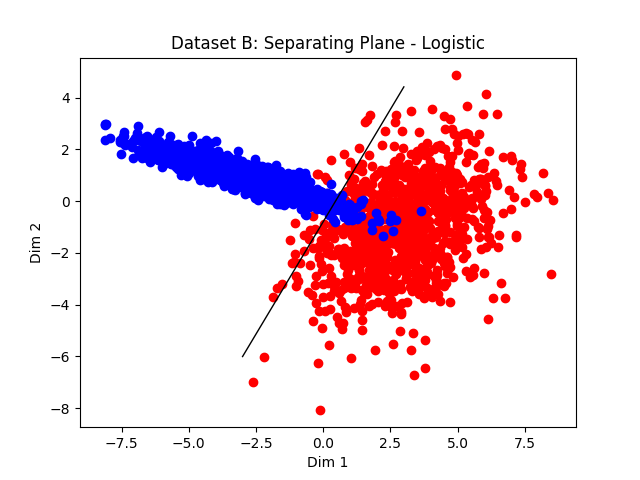
\includegraphics[width=.9\linewidth]{img_B_Log.png}
		\end{subfigure}
		\begin{subfigure}{.5\textwidth}
			\centering
			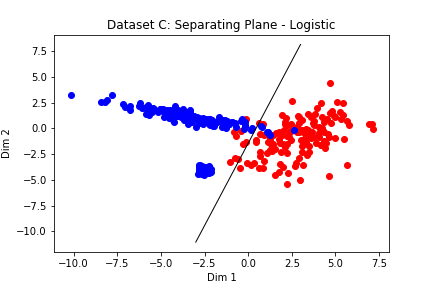
\includegraphics[width=.9\linewidth]{img_C_Log.png}
		\end{subfigure}
		\caption{Three different Datasets fit with IRLS estimates from Logistic Regression model. The seperating plane is in black.}
	\end{figure}
	
	\section{Linear Regression}
	We now implement linear regression by solving the normal equations. The estimated parameters are displayed in table 3.1. The corresponding decision boundary is presented in figure 3.1.
	
	\begin{table}
		\caption {Linear Regression Parameter Values} \label{tab:title} 
		\begin{center}		
			\begin{tabular}{*5l}   
				\toprule
				\emph{Dataset}&  $b$ & $w_1$  & $w_2$\\\midrule
				A & 0.492 & -0.373 & -0.264 \\ 
				B & 0.50 & -0.104 & 0.0518 \\
				C & 0.508 & -0.128 & -0.017 \\\bottomrule
				\hline
			\end{tabular}
		\end{center}
	\end{table}

\begin{figure}
	\begin{subfigure}{.5\textwidth}
		\centering
		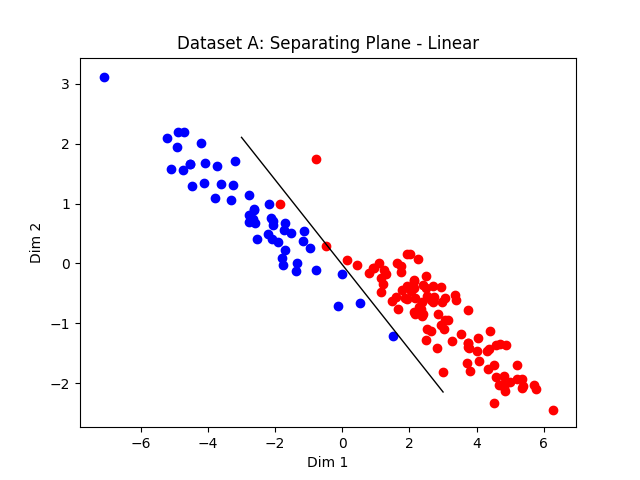
\includegraphics[width=.9\linewidth]{img_A_Lin.png}
	\end{subfigure}
	\begin{subfigure}{.5\textwidth}
		\centering
		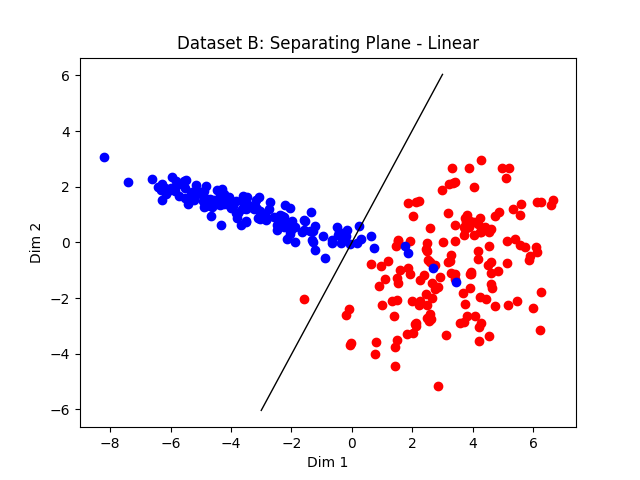
\includegraphics[width=.9\linewidth]{img_B_Lin.png}
	\end{subfigure}
	\begin{subfigure}{.5\textwidth}
		\centering
		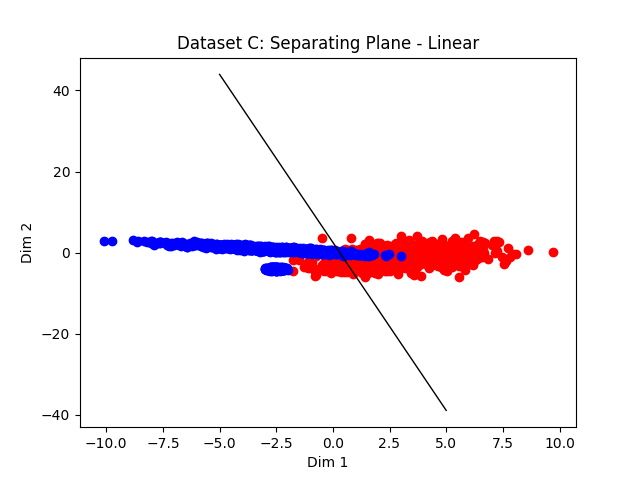
\includegraphics[width=.9\linewidth]{img_C_Lin.png}
	\end{subfigure}
	\caption{Three different Datasets fit with the Linear Regression model. The seperating plane is in black.}
\end{figure}

\newpage

\section{Comparing the Approaches}
We compute the misclassification error on the training and test data.
The results are presented in table 4.1.

	\begin{table}
		\caption {Test error for the models applied to the datasets, with ground truth values in brackets} \label{tab:title} 
		\begin{center}		
			\begin{tabular}{*5l}   
				\toprule
				Dataset &  LDA & Logistic & Linear
				\\\midrule
				A & 0.035 (0.013) & 0.029 (0.0067) & 0.0207 (0.0133) \\ 
				B & 0.0415 (0.03) & 0.043 (0.02) & 0.0415 (0.03) \\
				C & 0.039 (0.0575) & 0.0237 (0.0425) & 0.0423 (0.055) \\\bottomrule
				\hline
			\end{tabular}
		\end{center}
	\end{table}

For Dataset A, the Logistic and Linear models outperformed the MoG model, since the LDA prior shifted probability away from the class \(Y=1\) (since only one third of training examples were in this class). The other two models, which did not take into account the class imbalance, performed better. For B, the models performed similarily. It should be noted that the MoG and Linear models had identical performances. This is because the linear model and MoG produce the same decision boundary when the number of sample points is identical between classes [1]. For C, the logistic classifier  outperformed the other classifiers. Dataset C contained a class which was itself a Mixture of Gaussians, a clear violation of the data distribution assumptions that the LDA model relies on, but the Logistic model does not. Specifically, the LDA tried to fit the Mixture distribution as a single Gaussian, which resulted in a clearly bad fit (see bottom image of figures 1.1 and 5.1).

Generally, the misclassiffication error was smaller on the training versus the test data. This was expected, since the model parameters were fit to maximize the likelihood of the training data. Surprisingly, the test error for dataset C was lower than the training error.

\section{QDA Model}

	\begin{table}
		\caption {QDA Parameter Values} \label{tab:title} 
		\begin{center}		
			\begin{tabular}{*6l}   
				\toprule
				\emph{Data}&  $\pi$ & $\mu_1$  & $\mu_2$ & $\Sigma_1$ & $\Sigma_2$ \\\midrule
				A & 0.33 
				& $\begin{bmatrix}2.89 \\ -0.89\end{bmatrix}$ 
				& $\begin{bmatrix}-2.69 \\ 0.87\end{bmatrix}$ 
				& $\begin{bmatrix}
				2.31 & -1.05 \\
				-1.05 & 0.576 \\ \end{bmatrix}$
				& $\begin{bmatrix}
				2.70 & -1.30 \\
				-1.30 & 0.69 \\ \end{bmatrix}$			
				\\ \\
				B & 0.5 
				& $\begin{bmatrix}3.34 \\ -0.835\end{bmatrix}$ 
				& $\begin{bmatrix}-3.22 \\ 1.083\end{bmatrix}$ 
				& $\begin{bmatrix}
				2.54 & 1.064 \\
				1.064 & 2.96 \\ \end{bmatrix}$
				& $\begin{bmatrix}
				4.15 & -1.33 \\
				-1.33 & 0.516 \\ \end{bmatrix}$			
				\\ \\
				C & 0.625
				& $\begin{bmatrix}2.79 \\ -0.838\end{bmatrix}$ 
				& $\begin{bmatrix}-2.94 \\ -0.958\end{bmatrix}$ 
				& $\begin{bmatrix}
				2.90 & 1.25 \\
				1.25 &  2.92 \\ \end{bmatrix}$
				& $\begin{bmatrix}
				2.87 & -1.76 \\
				-1.76 & 6.56 \\ \end{bmatrix}$			
				\\\bottomrule
				\hline
			\end{tabular}
		\end{center}
	\end{table}

\begin{figure}
	\begin{subfigure}{.5\textwidth}
		\centering
		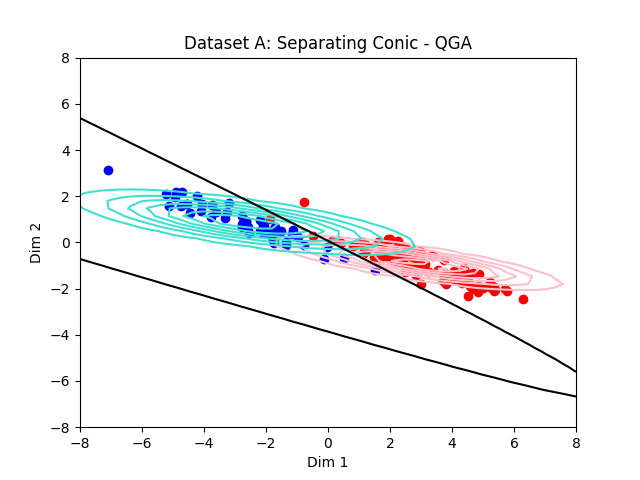
\includegraphics[width=.9\linewidth]{img_A_MoG_dm.png}
	\end{subfigure}
	\begin{subfigure}{.5\textwidth}
		\centering
		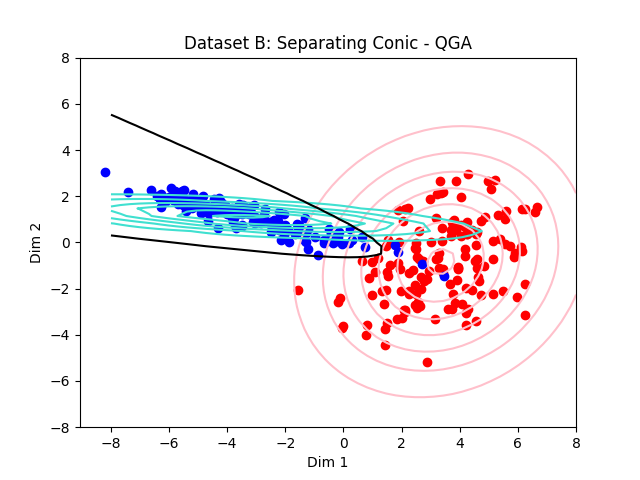
\includegraphics[width=.9\linewidth]{img_B_MoG_dm.png}
	\end{subfigure}
	\begin{subfigure}{.5\textwidth}
		\centering
		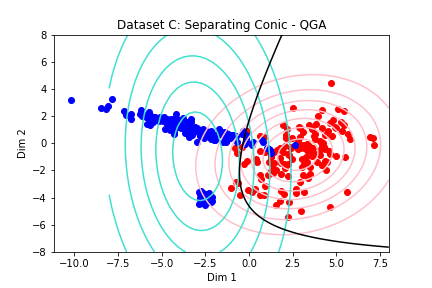
\includegraphics[width=.9\linewidth]{img_C_MoG_dm.png}
	\end{subfigure}
	\caption{Three different Datasets fit with the QDA model. The seperating conic is in black.}
\end{figure}

The estimated parameters for QDA are presented in table 5.1, and the misclassification error is presented in table 5.2.
As before, the error rate is higher then the test rate. The error rate is similar between QDA and LDA for dataset A. This was expected since the data generating distribution had a common covariance, and so the estimated \(\Sigma\)'s for each cluster were nearly identical, anyways. For datasets B and C, the QDA model had the lowest error rate. This makes sense since the true data generating distribution was a Mixture of Gaussians (with different \(\Sigma\)'s) 

	\begin{table}
		\caption {Test error for the QDA model applied to the datasets, with ground truth values in brackets} \label{tab:title} 
		\begin{center}		
			\begin{tabular}{*5l}   
				\toprule
				 A & B & C
				\\\midrule
				 0.0273 (0.013) & 0.02 (0.013) & 0.036 (0.05) \\\bottomrule
				\hline
			\end{tabular}
		\end{center}
	\end{table}

\newpage

\section{References}
[1] Hastie, T, Elements of Statistical Learning pg 100.


\end{document}